% PAKETE UND DOKUMENTKONFIGURATION
\documentclass[11pt, a4paper]{article}

% Encoding für Umlaute
\usepackage[utf8]{inputenc}
\usepackage[T1]{fontenc}

% Silbentrennung
\usepackage[ngerman]{babel}

% erweiterte Matheumgebungen und Formelnummer mit Sectionnummer
\usepackage{amsmath}
\numberwithin{equation}{section}

% Braket Notation
\usepackage{braket}
\usepackage{isotope}

% zusätzliche mathematische Schriftarten
\usepackage{amsfonts}

% verschiedene mathematische Symbole
\usepackage{amssymb}

% Einheiten setzen z.B. \SI{10}{\kilo\gram\meter\per\second\squared}
% Fehler: \SI{10 +- 0,2e-4}{\metre}
\usepackage{siunitx}
\sisetup{
  output-decimal-marker={,},
  separate-uncertainty
}

% Einheitendefinitionen
\DeclareSIUnit{\skt}{Skt.}

% Operatordefinitionen
\DeclareMathOperator{\erf}{erf}

% Randbreiten
\usepackage[left=3.5cm,right=3.5cm,top=3cm,bottom=3cm,twoside]{geometry}

% Bilder einfügen
\usepackage{graphicx}

% Verweise innerhalb des Dokuments
\usepackage{hyperref}
\hypersetup{
	colorlinks = true,
	allcolors = {black}
}

% bessere Tabellenlayouts
\usepackage{booktabs}
\usepackage{multirow}

% Seitenlayout (Kopfzeile)
\usepackage{fancyhdr}

% Float Barriers
\usepackage{placeins}

% Pakete für gedrehte Subfigures
\usepackage{caption}
\usepackage{subcaption}
\usepackage{rotating}

% Caption-Setup
\captionsetup{font={small}}
\renewcommand{\thefigure}{\thesection.\arabic{figure}}
\renewcommand{\thesubfigure}{\alph{subfigure}}
\renewcommand{\thetable}{\thesection.\arabic{table}}
\renewcommand{\thesubtable}{\alph{subtable}}

% Manuelle Silbentrennung
\hyphenation{Re-so-na-tor Mo-den-ab-stand Re-so-na-tor-län-ge}

% Tiefe des Inhaltsverzeichnisses (Level: 1 sections, 2 subsections,
% 3 subsubsections)
\setcounter{tocdepth}{3}

% FANCYHDR SETUP
\pagestyle{fancy}
\fancyhead[EL,OR]{\thepage}
\fancyhead[ER]{\leftmark}
\fancyhead[OL]{\rightmark}

\renewcommand{\sectionmark}[1]{
\markboth{\thesection{} #1}{\thesection{} #1}
}
\renewcommand{\subsectionmark}[1]{
\markright{\thesubsection{} #1}
}

% DOKUMENTINFORMATIONEN
\title{P523 \\ Beta Spektrometer}

\author{Christopher Deutsch\footnote{christopher.deutsch@uni-bonn.de} \and Christian Bespin\footnote{christian.bespin@uni-bonn.de}}

\date{\today}

\begin{document}

\begin{titlepage}

\maketitle

% DURCHFÜHRUNGSDATUM UND TUTOR
\begin{center}
\begin{tabular}{l r}
Durchführung: & 07./08. April 2015 \\
Gruppe: & $\alpha$ 6 \\
Tutor: & Yannick Wunderlich
\end{tabular}
\end{center}

% ZUSAMMENFASSUNG
\begin{abstract}
\noindent
\end{abstract}

\end{titlepage}

% INHALTSVERZEICHNIS
\tableofcontents
% Neue Seite nach TOC
\newpage

% INHALT VERSUCHSPROTOKOLL

\section{Einführung}

In diesem Praktikumsversuch werden Spektren und Maximalenergie der emittierten Teilchen verschiedener $\beta$-Strahler vermessen bzw. bestimmt.
Der $\beta$-Zerfall stellt eine Form der Kernumwandlung dar und sendet dabei Elektronen oder Positronen aus, die ein kontinuierliches Energiespektrum aufweisen, welches häufig auch diskrete, charakteristische Linien aufweist, die zur Kalibration des verwendeten Spektrometers genutzt werden.

\section{Theorie}
\subsection{$\beta$-Zerfall}
\begin{itemize}
	\item schwache WW
	\item Elementarvertex?
\end{itemize}

\subsubsection{Zerfallsarten}
Man unterscheidet zwischen drei verschiedenen $\beta$-Zerfallsarten ($m(A,Z)$: Atommasse, $Q$: Zerfallsenergie):
\begin{itemize}
	\item \textbf{Beta-Plus-Zerfall ($\beta^+$):}
	\begin{align}
	\mathrm{p} \to \mathrm{n} + \mathrm{e}^+ + \nu_\mathrm{e}
	\end{align}
	\begin{align}
		Q_{\beta^+} = m( A, Z ) - m( A, Z - 1) - 2 m_\mathrm{e}
	\end{align}
	
	\item \textbf{Beta-Minus-Zerfall ($\beta^-$):}
	\begin{align}
	\mathrm{n} \to \mathrm{p} + \mathrm{e}^- + \overline{\nu}_\mathrm{e}
	\end{align}
	\begin{align}
	Q_{\beta^-} = m( A, Z ) - m( A, Z + 1)
	\end{align}
	
	\item \textbf{Elektroneneinfang ($\epsilon$):}
	\begin{align}
	\mathrm{p} + \mathrm{e}^- \to \mathrm{n} + \nu_\mathrm{e}
	\end{align}
	\begin{align}
	Q_{\epsilon} = m( A, Z ) - m( A, Z - 1) - E_\mathrm{Bind.}
	\end{align}
	Nach dem Einfang befindet sich das Atom in einem angeregten Zustand, sodass zusätlich die Bindungsenergie des eingefangenen Elektrons abgezogen werden muss.
\end{itemize}
Grundsätzlich ist ein Zerfall nur möglich, wenn die Zerfallsenergie $Q$ positiv ist (Energieerhaltung).

\subsubsection{Fermitheorie des $\beta$-Zerfalls}
\begin{itemize}
	\item Einführung: historische Relevanz des kontinuierlichen Spektrums (Dreikörperzerfall und kein Zweikörperzerfall)
	\item Spektrum
	\item erlaubte Übergänge
	\item Kurieplot
	\item verbotene Übergänge
	\item Einfluß des Coulombfeldes
\end{itemize}

Spektrum nach Krane:
\begin{align}
	N(p) \propto p^2 \left( Q - T_\mathrm{e} \right)^2 F(Z, p) \left| M_{fi} \right|^2 S(p, q)
\end{align}

Aufpassen bei der Definition von $\epsilon_0$ im Kurie-Plot von Riezler-Kopitzki.
Da kann gut und gerne mal $\pm \SI{511}{\kilo\electronvolt}$ rauskommen wenn man die falsche Definition verwendet.

Man definiert:
\begin{align}
	\epsilon = 1 + \frac{E_\mathrm{kin}}{m_\mathrm{e} c^2} \\
	\eta = \frac{p}{m_\mathrm{e} c} \\
	\epsilon_0 = 1 + \frac{Q}{m_\mathrm{e} c^2} \\
\end{align}
Unsinnige Definition $\epsilon_0$ aber damit folgt Riezler-Kopitzki Form.

\begin{align}
	N(\epsilon) = N(p) \frac{\mathrm{d}p}{\mathrm{d}\epsilon}\propto N(p) \frac{\epsilon}{\eta}
\end{align}

\subsubsection{Innere Konversion und Augereffekt}

\subsection{Das $\beta$-Spektrometer}
Das Spektrometer ist ein Instrument, welches es ermöglicht, eine Vielzahl von Teilchen nach gewissen Eigenschaften wie zum Beispiel Energie, Impuls oder Masse zu trennen und dabei die Anzahl der auftretenden Teilchen in einem gewissen (Energie-, Impuls-, Massen-) Intervall zu zählen.
Den resultierenden Graphen nennt man ein Spektrum.

\subsubsection{Grundlagen}
In diesem Versuch wird ein magnetisches Spektrometer verwendet, welches die Ablenkung von geladenen Teilchen im Magnetfeld ausnutzt.
Betrachtet man ein Elektron, welches sich in einem homogenen Magnetfeld $\vec{B}$ mit der Geschwindigkeit $\vec{v}$ senkrecht zum Magnetfeld bewegt, so wirkt die Lorentzkraft als Zentripetalkraft und das Elektron beschreibt eine Kreisbahn mit Radius $\rho$.
\begin{align}
	F_\mathrm{Z} &\stackrel{!}{=} F_\mathrm{L} \nonumber\\
	e v B &= \frac{\gamma m_\mathrm{e} v^2}{\rho}
\end{align}
Mit dem relativistischem Impuls $p = \gamma m v$ folgt sofort:
\begin{align}
	p = e B \rho
	\label{eq:impuls_radius}
\end{align}
Man sieht, dass die Größe $B \rho$ charakteristisch für den Impuls ist und gleichzeitig eine Aussage über die Dimension des Spektrometers macht.
Daher werden Impulse in der $\beta$-Spektroskopie als $B \rho$-Werte angegeben.

(Kram für eventuell verwendete einheitenlose Größen $\epsilon$, $\eta$, wasweißich)

\begin{align}
	B \rho = \frac{1}{c e} \sqrt{T \left( 2 E_0 + T \right)}
	\label{eq:b_rho}
\end{align}

\subsubsection{Halbkreisförmiges Spektrometer}
(GRAFIK)
Ein halbkreisförmiges Spektrometer nutzt ein homogenes Magnetfeld senkrecht zur Flugrichtung der Elektronen um diese auf eine Kreisbahn zu lenken.
Nach Gleichung \eqref{eq:impuls_radius} ist das Produkt von Magnetfeld $B$ und Bahnradius $\rho$ charakteristisch für den Impuls des Elektrons.

Nachteil nur Fokussierung in der $\rho$-Ebene führt zu geringer Transmission.
Vorteil: einfache Konstruktion, Magnetfeld leicht zu messen, gut geeignet um große Spektralbereiche aufzunehmen (konstante Magnetfeldstärke)

\subsubsection{Doppelt-fokussierendes Spektrometer}
(GRAFIK)
Betatron-Oszillationen ($\omega_0$: Elektronen Umlauffrequenz) (Zitat Hillert)
\begin{align}
	\omega_\rho = \omega_0 \sqrt{1-n} \qquad \omega_z = \omega_0 \sqrt{n}
\end{align}
mit dem Feldindex:
\begin{align}
	n = - \frac{\rho}{B_z(\rho)} \frac{\mathrm{d} B_z(\rho)}{\mathrm{d} \rho}
\end{align}
Während einer halben Periode der jeweiligen Betatronschwingung läuft das Elektron auf der Kreisbahn einen Winkel von:
\begin{align}
	\phi_\rho &= \omega_0 \cdot \frac{\pi}{\omega_\rho} & \phi_z &= \omega_0 \cdot \frac{\pi}{\omega_z}\\
	\phi_\rho &= \pi \left[ 1+ \frac{\rho_0 B^\prime(\rho_0)}{B(\rho_0)} \right]^{-\frac{1}{2}} & \phi_z &= \pi \left[ -\frac{\rho_0 B^\prime(\rho_0)}{B(\rho_0)} \right]^{-\frac{1}{2}} \label{eq:betatronwinkel}
\end{align}
ab, wobei $\rho_0$ den Designorbit kennzeichnet.
An Gleichung \eqref{eq:betatronwinkel} ließt man nach quadrieren ab:
\begin{align}
	\frac{1}{\phi_\rho^2} + \frac{1}{\phi_z^2} = \frac{1}{\pi^2} \label{eq:betatronwinkelverhaeltnis}
\end{align}
Um eine stigmatische Abbildung zu erlangen, das heißt der Fokus der $\rho$ und der $z$-Ebene liegen im selben Punkt, muss die Bedingung $\phi_\rho = \phi_z$ gestellt werden.
Damit folgt aus Gleichung \eqref{eq:betatronwinkelverhaeltnis} der gesamte Winkel der Elektronenbahn im Spektrometer.
Dieser ergibt sich zu $\phi = \pi \sqrt{2}$, weshalb das doppelt-fokussierende Spektrometer auch $\pi \sqrt{2}$-Spektrometer genannt wird.
Gleichzeitig folgt aus der gestellten Anforderung $\phi_\rho = \phi_z$ mit Gleichung \eqref{eq:betatronwinkel} die Bestimmungsgleichung für das magnetische Feld:
\begin{align}
	B^\prime(\rho) = - \frac{1}{2 \rho} B(\rho)
\end{align}
Mit der Randbedingung $B(\rho_0) = B_0$ folgt als allgemeine Lösung:
\begin{align}
	B(\rho) = B_0 \sqrt{\frac{\rho_0}{\rho}}
\end{align}
Der Vorteil gegenüber dem halbkreisförmigen Spektrometer liegt darin, dass das doppelt-fokussierende ebenfalls in der $z$-Ebene fokussierend wirkt und damit höhere Transmissionen möglich sind.

\subsection{Detektoren (?)}
\subsubsection{Halbleiterdetektoren}

\subsubsection{Hallsonde}

\subsubsection{Hysterese (?)}


\section{Durchführung und Auswertung}
Die ausführliche Durchführung ist der Versuchsanleitung \cite{anleitung} zu entnehmen.
Sollten Abweichungen bei der Durchführung auftreten, so werden diese im jeweiligen Unterkapitel dargestellt.

\subsection{Bestimmung der Offsetspannung der Hallsonde}

Zur Messung des Magnetfelds des Spektrometers wird eine Hallsonde verwendet, die jedoch auch bei ausgeschaltetem Magnetfeld eine Spannung $\neq 0$ \si{\volt} anzeigt.
Um die tatsächliche Offsetspannung zu ermitteln, nutzt man die Hysterese des Magneten aus und misst für beide Stromrichtungen, die am Magneten angelegt werden die jeweiligen Remanenzfelder (als Hallspannung $U_\text{H}$) gemessen.
\begin{figure}[h]
	\centering
	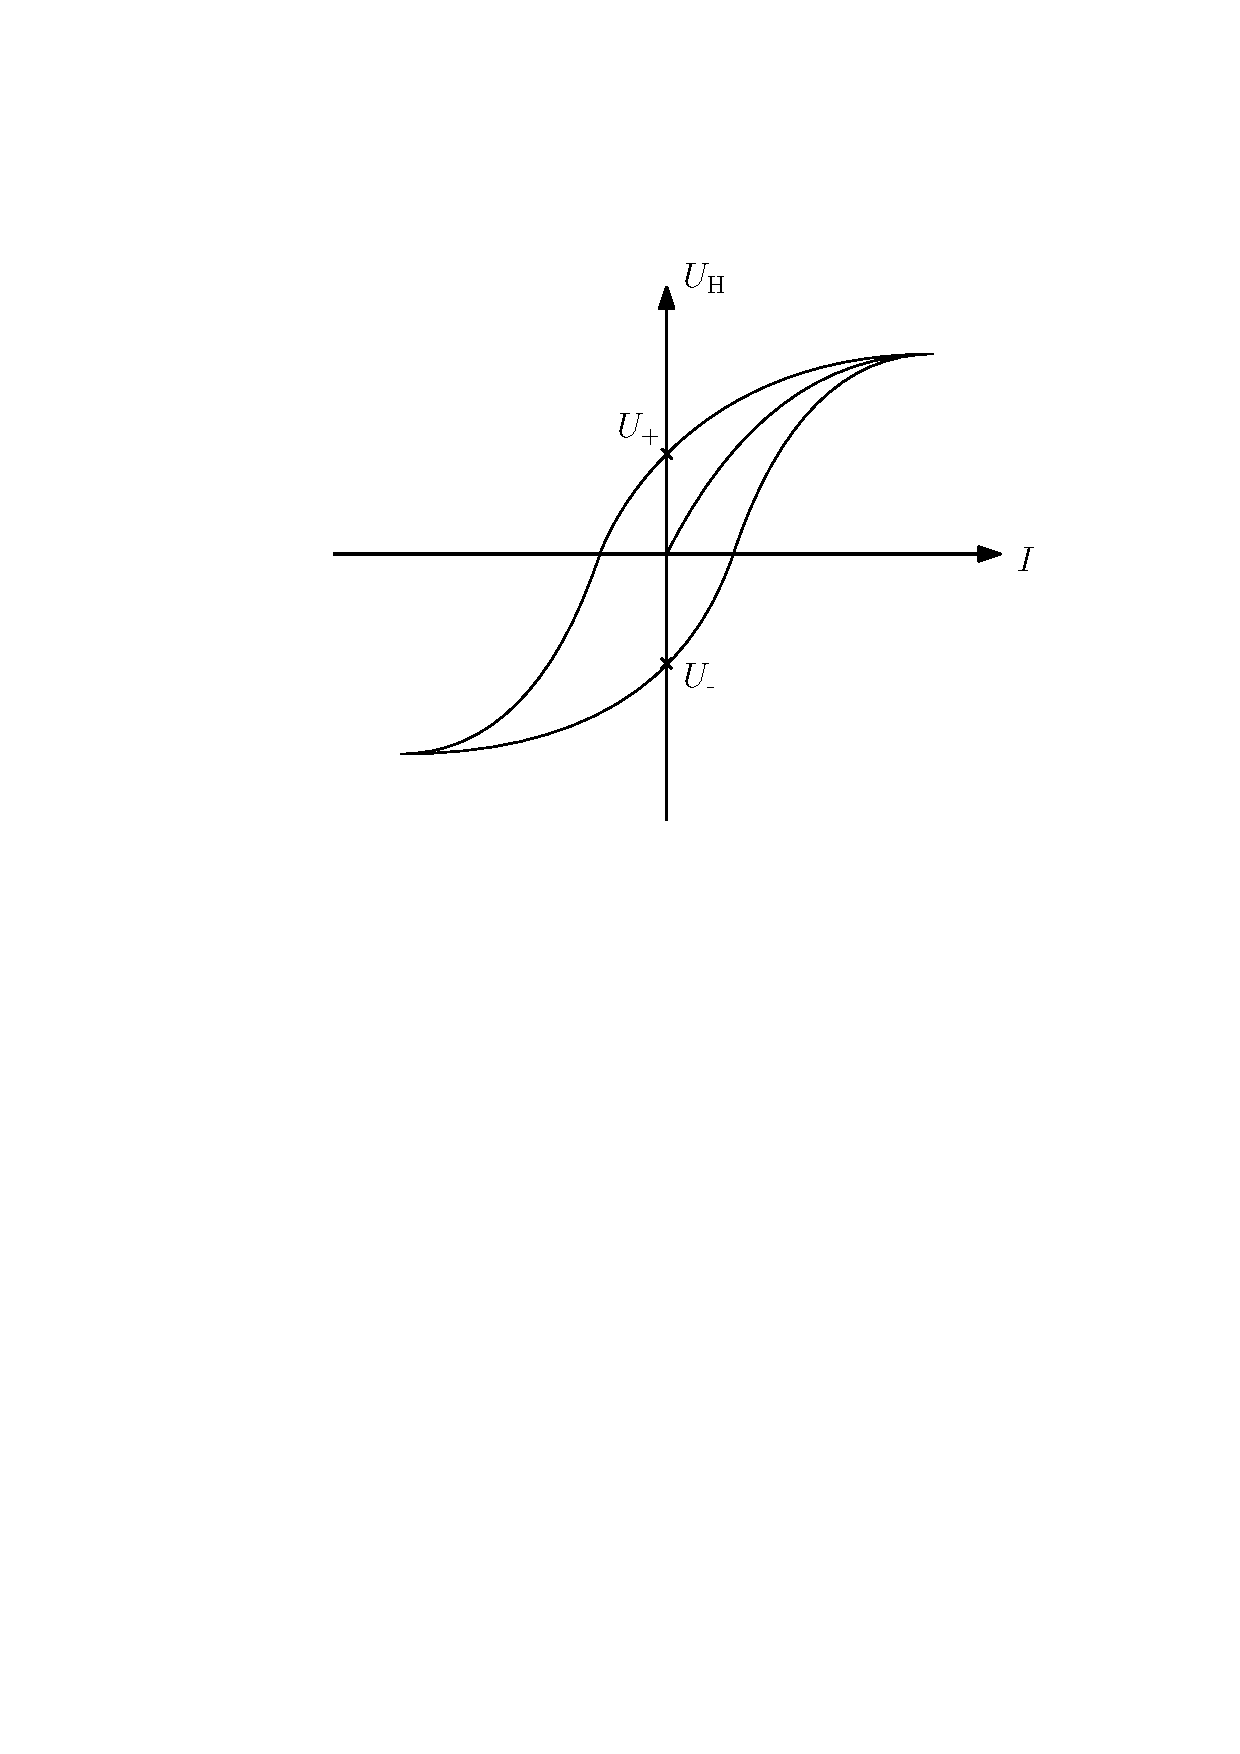
\includegraphics[width=0.5\textwidth]{./figures/hysterese.pdf}
	\caption{Skizzierte Hysteresekurve. Der tatsächliche Spannungswert für $I=\SI{0}{\ampere}$ ergibt sich aus Mittelung von $U_\text{+}$ und $U_\text{-}$.}
	\label{fig:hysterese}
\end{figure}
Bei jeder Messung wird dann das arithmetische Mittel (mit $U_0$ bezeichnet) von $U_\text{+}$ und $U_\text{-}$ berechnet und im Anschluss über alle $U_0$ wieder gemittelt, um einen guten Wert für die Offsetspannung $U_0$ zu erhalten.
\begin{table}[h]
	\centering
	\begin{tabular}{SSSSSSS}
\toprule
{$U_+$ / \si{\skt}} & {$\Delta U_+$ / \si{\skt}} & {$U_-$ / \si{\skt}} & {$\Delta U_-$ / \si{\skt}} &  & {$U_0$ / \si{\skt}} & {$\Delta U_0$ / \si{\skt}} \\ \midrule
9.4 & 0.1    & 5.0 & 0.1    &  & 7.20   & 0.08   \\
9.4 & 0.1    & 5.0 & 0.1    &  & 7.20   & 0.08   \\
9.3 & 0.1    & 5.0 & 0.1    &  & 7.15   & 0.08   \\
9.3 & 0.1    & 5.0 & 0.1    &  & 7.15   & 0.08   \\
9.3 & 0.1    & 4.9 & 0.1    &  & 7.10   & 0.08   \\
9.3 & 0.1    & 5.0 & 0.1    &  & 7.15   & 0.08   \\ \midrule
    &        &     & {$\overline{U_0}$ / \si{\skt}:}    &  & 7.16   & 0.04   \\ \bottomrule
\end{tabular}
	\caption{Messwerte und Auswertung zur Bestimmung der Offsetspannung der Hallsonde. Die unterste Zeile ergibt sich aus Mittelung über alle $U_0$.}
	\label{tab:offset}
\end{table}
Der Fehler der Mittelung über $U_\text{+}$ und $U_\text{-}$ ergibt sich mit Gauß'scher Fehlerfortpflanzung aus
\begin{align}
	\Delta U_0 = \sqrt{(\Delta U_\text{+})^2 + (\Delta U_\text{-})^2}
\end{align}
Den im weiteren Verlauf benutzten Wert für die Offsetspannung $\overline{U_0}$ erhält man, indem über alle $U_0$ gemittelt wird. Da die Fehler auf $U_0$ gleich groß sind, ergibt sich für $\Delta\overline{U_0}$
\begin{align}
	\Delta\overline{U_0} = \frac{\Delta U_0}{\sqrt{6}}
\end{align}
und alle gemessenen Hallspannungen werden in der folgenden Auswertung um
\begin{align}
	\overline{U_0} = \SI{7.16 +- 0.03}{\skt}
\end{align}
korrigiert.

\subsection{Kalibration des Spektrometers}
Kalibration mit \isotope[137]{Ba}.
Fehler der Hallspannung:
\begin{align}
	\Delta U_\mathrm{H} = \SI{0.1}{\skt}
\end{align}
Korrektur der Hallspannung:
\begin{align}
	U_\mathrm{H}^\mathrm{Korr} &= U_\mathrm{H} - U_0 \\
	\Delta U_\mathrm{H}^\mathrm{Korr} &= \sqrt{\Delta U_\mathrm{H}^2 + \Delta U_0^2}
\end{align}
Fehler der Counts (Poisson-Verteilung):
\begin{align}
	\Delta N = \sqrt{N}
\end{align}
Abzug des Hintergrundes:
\begin{align}
	N - N_\mathrm{HG} \qquad \Delta(N - N_\mathrm{HG}) = \sqrt{\Delta N^2 + \Delta N_\mathrm{HG}^2}
\end{align}
Korrektur der Dispersion (das gemessene Impulsintervall ist proportional zum Magnetfeld):
\begin{align}
	n = \frac{N-N_\mathrm{HG}}{U_\mathrm{H}^\mathrm{Korr}}
\end{align}
(TODO: $n$ anderen Namen geben und physikalische Bedeutung klarmachen; keine Counts mehr sondern jetzt eher eine Impulsverteilung)

Aus den gegebenen Bindungsenergien:
\begin{align*}
	E_\mathrm{K} = \SI{37,441}{\kilo\electronvolt}
\end{align*}
und
\begin{align*}
	E_{\mathrm{L}_{\mathrm{I}}} = \SI{5,987}{\kilo\electronvolt} \\
	E_{\mathrm{L}_{\mathrm{II}}} = \SI{5,624}{\kilo\electronvolt} \\
	E_{\mathrm{L}_{\mathrm{III}}} = \SI{5,247}{\kilo\electronvolt}
\end{align*}
Entartungsgrade:
\begin{align*}
	g_{\mathrm{L}_{\mathrm{I}}} = \num{1} \\
	g_{\mathrm{L}_{\mathrm{II}}} = \num{2} \\
	g_{\mathrm{L}_{\mathrm{III}}} = \num{1}
\end{align*}
Gewichtetes Mittel:
\begin{align}
	E_\mathrm{L} = \frac{E_{\mathrm{L}_{\mathrm{I}}} + 2E_{\mathrm{L}_{\mathrm{II}}} + E_{\mathrm{L}_{\mathrm{III}}}}{4} \approx \SI{5,621}{\kilo\electronvolt}
\end{align}

Bestimmung der $B\rho$-Werte zur Kalibration aus Gleichung \ref{eq:b_rho}, wobei für die kinetische Energie $T$ des Elektrons die Differenz von Anregung $Q = \SI{661,660}{\kilo\electronvolt}$ und Bindungsenergie genommen wird:
\begin{align}
	\left(B \rho \right)_\mathrm{K} = \SI{3379}{G.cm} \\
	\left(B \rho \right)_\mathrm{L} = \SI{3497}{G.cm}
\end{align}


\subsubsection{Grobspektrum von Barium}
\begin{figure}
	\centering
	% GNUPLOT: LaTeX picture with Postscript
\begingroup
  \makeatletter
  \providecommand\color[2][]{%
    \GenericError{(gnuplot) \space\space\space\@spaces}{%
      Package color not loaded in conjunction with
      terminal option `colourtext'%
    }{See the gnuplot documentation for explanation.%
    }{Either use 'blacktext' in gnuplot or load the package
      color.sty in LaTeX.}%
    \renewcommand\color[2][]{}%
  }%
  \providecommand\includegraphics[2][]{%
    \GenericError{(gnuplot) \space\space\space\@spaces}{%
      Package graphicx or graphics not loaded%
    }{See the gnuplot documentation for explanation.%
    }{The gnuplot epslatex terminal needs graphicx.sty or graphics.sty.}%
    \renewcommand\includegraphics[2][]{}%
  }%
  \providecommand\rotatebox[2]{#2}%
  \@ifundefined{ifGPcolor}{%
    \newif\ifGPcolor
    \GPcolortrue
  }{}%
  \@ifundefined{ifGPblacktext}{%
    \newif\ifGPblacktext
    \GPblacktexttrue
  }{}%
  % define a \g@addto@macro without @ in the name:
  \let\gplgaddtomacro\g@addto@macro
  % define empty templates for all commands taking text:
  \gdef\gplbacktext{}%
  \gdef\gplfronttext{}%
  \makeatother
  \ifGPblacktext
    % no textcolor at all
    \def\colorrgb#1{}%
    \def\colorgray#1{}%
  \else
    % gray or color?
    \ifGPcolor
      \def\colorrgb#1{\color[rgb]{#1}}%
      \def\colorgray#1{\color[gray]{#1}}%
      \expandafter\def\csname LTw\endcsname{\color{white}}%
      \expandafter\def\csname LTb\endcsname{\color{black}}%
      \expandafter\def\csname LTa\endcsname{\color{black}}%
      \expandafter\def\csname LT0\endcsname{\color[rgb]{1,0,0}}%
      \expandafter\def\csname LT1\endcsname{\color[rgb]{0,1,0}}%
      \expandafter\def\csname LT2\endcsname{\color[rgb]{0,0,1}}%
      \expandafter\def\csname LT3\endcsname{\color[rgb]{1,0,1}}%
      \expandafter\def\csname LT4\endcsname{\color[rgb]{0,1,1}}%
      \expandafter\def\csname LT5\endcsname{\color[rgb]{1,1,0}}%
      \expandafter\def\csname LT6\endcsname{\color[rgb]{0,0,0}}%
      \expandafter\def\csname LT7\endcsname{\color[rgb]{1,0.3,0}}%
      \expandafter\def\csname LT8\endcsname{\color[rgb]{0.5,0.5,0.5}}%
    \else
      % gray
      \def\colorrgb#1{\color{black}}%
      \def\colorgray#1{\color[gray]{#1}}%
      \expandafter\def\csname LTw\endcsname{\color{white}}%
      \expandafter\def\csname LTb\endcsname{\color{black}}%
      \expandafter\def\csname LTa\endcsname{\color{black}}%
      \expandafter\def\csname LT0\endcsname{\color{black}}%
      \expandafter\def\csname LT1\endcsname{\color{black}}%
      \expandafter\def\csname LT2\endcsname{\color{black}}%
      \expandafter\def\csname LT3\endcsname{\color{black}}%
      \expandafter\def\csname LT4\endcsname{\color{black}}%
      \expandafter\def\csname LT5\endcsname{\color{black}}%
      \expandafter\def\csname LT6\endcsname{\color{black}}%
      \expandafter\def\csname LT7\endcsname{\color{black}}%
      \expandafter\def\csname LT8\endcsname{\color{black}}%
    \fi
  \fi
    \setlength{\unitlength}{0.0500bp}%
    \ifx\gptboxheight\undefined%
      \newlength{\gptboxheight}%
      \newlength{\gptboxwidth}%
      \newsavebox{\gptboxtext}%
    \fi%
    \setlength{\fboxrule}{0.5pt}%
    \setlength{\fboxsep}{1pt}%
\begin{picture}(7200.00,5040.00)%
    \gplgaddtomacro\gplbacktext{%
      \csname LTb\endcsname%
      \put(946,704){\makebox(0,0)[r]{\strut{}$-0{,}5$}}%
      \csname LTb\endcsname%
      \put(946,1518){\makebox(0,0)[r]{\strut{}$0$}}%
      \csname LTb\endcsname%
      \put(946,2332){\makebox(0,0)[r]{\strut{}$0{,}5$}}%
      \csname LTb\endcsname%
      \put(946,3147){\makebox(0,0)[r]{\strut{}$1$}}%
      \csname LTb\endcsname%
      \put(946,3961){\makebox(0,0)[r]{\strut{}$1{,}5$}}%
      \csname LTb\endcsname%
      \put(946,4775){\makebox(0,0)[r]{\strut{}$2$}}%
      \csname LTb\endcsname%
      \put(1078,484){\makebox(0,0){\strut{}$0$}}%
      \csname LTb\endcsname%
      \put(1651,484){\makebox(0,0){\strut{}$20$}}%
      \csname LTb\endcsname%
      \put(2223,484){\makebox(0,0){\strut{}$40$}}%
      \csname LTb\endcsname%
      \put(2796,484){\makebox(0,0){\strut{}$60$}}%
      \csname LTb\endcsname%
      \put(3368,484){\makebox(0,0){\strut{}$80$}}%
      \csname LTb\endcsname%
      \put(3941,484){\makebox(0,0){\strut{}$100$}}%
      \csname LTb\endcsname%
      \put(4513,484){\makebox(0,0){\strut{}$120$}}%
      \csname LTb\endcsname%
      \put(5086,484){\makebox(0,0){\strut{}$140$}}%
      \csname LTb\endcsname%
      \put(5658,484){\makebox(0,0){\strut{}$160$}}%
      \csname LTb\endcsname%
      \put(6231,484){\makebox(0,0){\strut{}$180$}}%
      \csname LTb\endcsname%
      \put(6803,484){\makebox(0,0){\strut{}$200$}}%
    }%
    \gplgaddtomacro\gplfronttext{%
      \csname LTb\endcsname%
      \put(176,2739){\rotatebox{-270}{\makebox(0,0){\strut{}$n$}}}%
      \put(3940,154){\makebox(0,0){\strut{}$U_\mathrm{H}$ / \si{\skt}}}%
      \csname LTb\endcsname%
      \put(5816,4602){\makebox(0,0)[r]{\strut{}Messwerte}}%
    }%
    \gplbacktext
    \put(0,0){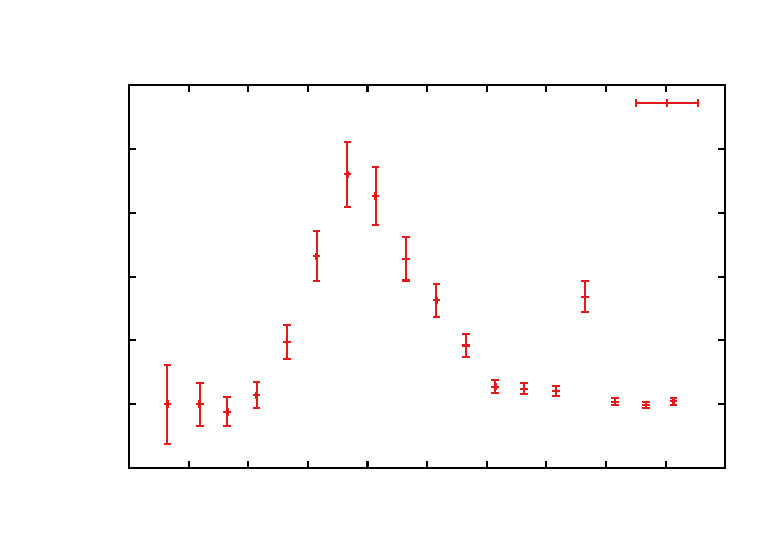
\includegraphics{./plots/barium_t4_grob}}%
    \gplfronttext
  \end{picture}%
\endgroup

	\caption{Barium Grobspektrum Transmission 4}
	\label{fig:ba_t4_grob}
\end{figure}
\begin{figure}
	\centering
	% GNUPLOT: LaTeX picture with Postscript
\begingroup
  \makeatletter
  \providecommand\color[2][]{%
    \GenericError{(gnuplot) \space\space\space\@spaces}{%
      Package color not loaded in conjunction with
      terminal option `colourtext'%
    }{See the gnuplot documentation for explanation.%
    }{Either use 'blacktext' in gnuplot or load the package
      color.sty in LaTeX.}%
    \renewcommand\color[2][]{}%
  }%
  \providecommand\includegraphics[2][]{%
    \GenericError{(gnuplot) \space\space\space\@spaces}{%
      Package graphicx or graphics not loaded%
    }{See the gnuplot documentation for explanation.%
    }{The gnuplot epslatex terminal needs graphicx.sty or graphics.sty.}%
    \renewcommand\includegraphics[2][]{}%
  }%
  \providecommand\rotatebox[2]{#2}%
  \@ifundefined{ifGPcolor}{%
    \newif\ifGPcolor
    \GPcolortrue
  }{}%
  \@ifundefined{ifGPblacktext}{%
    \newif\ifGPblacktext
    \GPblacktexttrue
  }{}%
  % define a \g@addto@macro without @ in the name:
  \let\gplgaddtomacro\g@addto@macro
  % define empty templates for all commands taking text:
  \gdef\gplbacktext{}%
  \gdef\gplfronttext{}%
  \makeatother
  \ifGPblacktext
    % no textcolor at all
    \def\colorrgb#1{}%
    \def\colorgray#1{}%
  \else
    % gray or color?
    \ifGPcolor
      \def\colorrgb#1{\color[rgb]{#1}}%
      \def\colorgray#1{\color[gray]{#1}}%
      \expandafter\def\csname LTw\endcsname{\color{white}}%
      \expandafter\def\csname LTb\endcsname{\color{black}}%
      \expandafter\def\csname LTa\endcsname{\color{black}}%
      \expandafter\def\csname LT0\endcsname{\color[rgb]{1,0,0}}%
      \expandafter\def\csname LT1\endcsname{\color[rgb]{0,1,0}}%
      \expandafter\def\csname LT2\endcsname{\color[rgb]{0,0,1}}%
      \expandafter\def\csname LT3\endcsname{\color[rgb]{1,0,1}}%
      \expandafter\def\csname LT4\endcsname{\color[rgb]{0,1,1}}%
      \expandafter\def\csname LT5\endcsname{\color[rgb]{1,1,0}}%
      \expandafter\def\csname LT6\endcsname{\color[rgb]{0,0,0}}%
      \expandafter\def\csname LT7\endcsname{\color[rgb]{1,0.3,0}}%
      \expandafter\def\csname LT8\endcsname{\color[rgb]{0.5,0.5,0.5}}%
    \else
      % gray
      \def\colorrgb#1{\color{black}}%
      \def\colorgray#1{\color[gray]{#1}}%
      \expandafter\def\csname LTw\endcsname{\color{white}}%
      \expandafter\def\csname LTb\endcsname{\color{black}}%
      \expandafter\def\csname LTa\endcsname{\color{black}}%
      \expandafter\def\csname LT0\endcsname{\color{black}}%
      \expandafter\def\csname LT1\endcsname{\color{black}}%
      \expandafter\def\csname LT2\endcsname{\color{black}}%
      \expandafter\def\csname LT3\endcsname{\color{black}}%
      \expandafter\def\csname LT4\endcsname{\color{black}}%
      \expandafter\def\csname LT5\endcsname{\color{black}}%
      \expandafter\def\csname LT6\endcsname{\color{black}}%
      \expandafter\def\csname LT7\endcsname{\color{black}}%
      \expandafter\def\csname LT8\endcsname{\color{black}}%
    \fi
  \fi
    \setlength{\unitlength}{0.0500bp}%
    \ifx\gptboxheight\undefined%
      \newlength{\gptboxheight}%
      \newlength{\gptboxwidth}%
      \newsavebox{\gptboxtext}%
    \fi%
    \setlength{\fboxrule}{0.5pt}%
    \setlength{\fboxsep}{1pt}%
\begin{picture}(7200.00,5040.00)%
    \gplgaddtomacro\gplbacktext{%
      \csname LTb\endcsname%
      \put(814,704){\makebox(0,0)[r]{\strut{}$0$}}%
      \put(814,1286){\makebox(0,0)[r]{\strut{}$0{,}2$}}%
      \put(814,1867){\makebox(0,0)[r]{\strut{}$0{,}4$}}%
      \put(814,2449){\makebox(0,0)[r]{\strut{}$0{,}6$}}%
      \put(814,3030){\makebox(0,0)[r]{\strut{}$0{,}8$}}%
      \put(814,3612){\makebox(0,0)[r]{\strut{}$1$}}%
      \put(814,4193){\makebox(0,0)[r]{\strut{}$1{,}2$}}%
      \put(814,4775){\makebox(0,0)[r]{\strut{}$1{,}4$}}%
      \put(1434,484){\makebox(0,0){\strut{}$148$}}%
      \put(2410,484){\makebox(0,0){\strut{}$150$}}%
      \put(3386,484){\makebox(0,0){\strut{}$152$}}%
      \put(4363,484){\makebox(0,0){\strut{}$154$}}%
      \put(5339,484){\makebox(0,0){\strut{}$156$}}%
      \put(6315,484){\makebox(0,0){\strut{}$158$}}%
    }%
    \gplgaddtomacro\gplfronttext{%
      \csname LTb\endcsname%
      \put(176,2739){\rotatebox{-270}{\makebox(0,0){\strut{}$n$}}}%
      \put(3874,154){\makebox(0,0){\strut{}$U_\mathrm{H}$ / \si{\skt}}}%
      \csname LTb\endcsname%
      \put(5816,4602){\makebox(0,0)[r]{\strut{}Messwerte}}%
      \csname LTb\endcsname%
      \put(5816,4382){\makebox(0,0)[r]{\strut{}g(x)}}%
    }%
    \gplbacktext
    \put(0,0){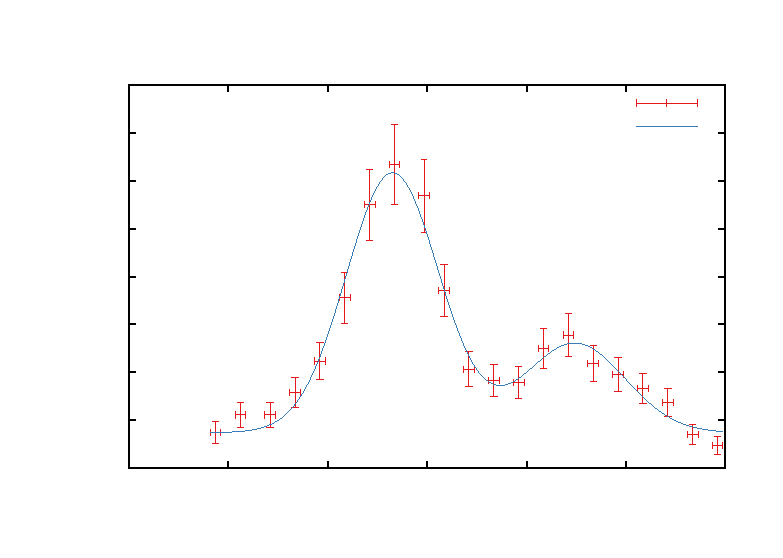
\includegraphics{./plots/barium_t4_fein}}%
    \gplfronttext
  \end{picture}%
\endgroup

	\caption{Barium Feinspektrum Transmission 4}
	\label{fig:ba_t4_grob}
\end{figure}
\begin{figure}
	\centering
	% GNUPLOT: LaTeX picture with Postscript
\begingroup
  \makeatletter
  \providecommand\color[2][]{%
    \GenericError{(gnuplot) \space\space\space\@spaces}{%
      Package color not loaded in conjunction with
      terminal option `colourtext'%
    }{See the gnuplot documentation for explanation.%
    }{Either use 'blacktext' in gnuplot or load the package
      color.sty in LaTeX.}%
    \renewcommand\color[2][]{}%
  }%
  \providecommand\includegraphics[2][]{%
    \GenericError{(gnuplot) \space\space\space\@spaces}{%
      Package graphicx or graphics not loaded%
    }{See the gnuplot documentation for explanation.%
    }{The gnuplot epslatex terminal needs graphicx.sty or graphics.sty.}%
    \renewcommand\includegraphics[2][]{}%
  }%
  \providecommand\rotatebox[2]{#2}%
  \@ifundefined{ifGPcolor}{%
    \newif\ifGPcolor
    \GPcolortrue
  }{}%
  \@ifundefined{ifGPblacktext}{%
    \newif\ifGPblacktext
    \GPblacktexttrue
  }{}%
  % define a \g@addto@macro without @ in the name:
  \let\gplgaddtomacro\g@addto@macro
  % define empty templates for all commands taking text:
  \gdef\gplbacktext{}%
  \gdef\gplfronttext{}%
  \makeatother
  \ifGPblacktext
    % no textcolor at all
    \def\colorrgb#1{}%
    \def\colorgray#1{}%
  \else
    % gray or color?
    \ifGPcolor
      \def\colorrgb#1{\color[rgb]{#1}}%
      \def\colorgray#1{\color[gray]{#1}}%
      \expandafter\def\csname LTw\endcsname{\color{white}}%
      \expandafter\def\csname LTb\endcsname{\color{black}}%
      \expandafter\def\csname LTa\endcsname{\color{black}}%
      \expandafter\def\csname LT0\endcsname{\color[rgb]{1,0,0}}%
      \expandafter\def\csname LT1\endcsname{\color[rgb]{0,1,0}}%
      \expandafter\def\csname LT2\endcsname{\color[rgb]{0,0,1}}%
      \expandafter\def\csname LT3\endcsname{\color[rgb]{1,0,1}}%
      \expandafter\def\csname LT4\endcsname{\color[rgb]{0,1,1}}%
      \expandafter\def\csname LT5\endcsname{\color[rgb]{1,1,0}}%
      \expandafter\def\csname LT6\endcsname{\color[rgb]{0,0,0}}%
      \expandafter\def\csname LT7\endcsname{\color[rgb]{1,0.3,0}}%
      \expandafter\def\csname LT8\endcsname{\color[rgb]{0.5,0.5,0.5}}%
    \else
      % gray
      \def\colorrgb#1{\color{black}}%
      \def\colorgray#1{\color[gray]{#1}}%
      \expandafter\def\csname LTw\endcsname{\color{white}}%
      \expandafter\def\csname LTb\endcsname{\color{black}}%
      \expandafter\def\csname LTa\endcsname{\color{black}}%
      \expandafter\def\csname LT0\endcsname{\color{black}}%
      \expandafter\def\csname LT1\endcsname{\color{black}}%
      \expandafter\def\csname LT2\endcsname{\color{black}}%
      \expandafter\def\csname LT3\endcsname{\color{black}}%
      \expandafter\def\csname LT4\endcsname{\color{black}}%
      \expandafter\def\csname LT5\endcsname{\color{black}}%
      \expandafter\def\csname LT6\endcsname{\color{black}}%
      \expandafter\def\csname LT7\endcsname{\color{black}}%
      \expandafter\def\csname LT8\endcsname{\color{black}}%
    \fi
  \fi
    \setlength{\unitlength}{0.0500bp}%
    \ifx\gptboxheight\undefined%
      \newlength{\gptboxheight}%
      \newlength{\gptboxwidth}%
      \newsavebox{\gptboxtext}%
    \fi%
    \setlength{\fboxrule}{0.5pt}%
    \setlength{\fboxsep}{1pt}%
\begin{picture}(7200.00,5040.00)%
    \gplgaddtomacro\gplbacktext{%
      \csname LTb\endcsname%
      \put(814,704){\makebox(0,0)[r]{\strut{}$0$}}%
      \csname LTb\endcsname%
      \put(814,1156){\makebox(0,0)[r]{\strut{}$20$}}%
      \csname LTb\endcsname%
      \put(814,1609){\makebox(0,0)[r]{\strut{}$40$}}%
      \csname LTb\endcsname%
      \put(814,2061){\makebox(0,0)[r]{\strut{}$60$}}%
      \csname LTb\endcsname%
      \put(814,2513){\makebox(0,0)[r]{\strut{}$80$}}%
      \csname LTb\endcsname%
      \put(814,2966){\makebox(0,0)[r]{\strut{}$100$}}%
      \csname LTb\endcsname%
      \put(814,3418){\makebox(0,0)[r]{\strut{}$120$}}%
      \csname LTb\endcsname%
      \put(814,3870){\makebox(0,0)[r]{\strut{}$140$}}%
      \csname LTb\endcsname%
      \put(814,4323){\makebox(0,0)[r]{\strut{}$160$}}%
      \csname LTb\endcsname%
      \put(814,4775){\makebox(0,0)[r]{\strut{}$180$}}%
      \csname LTb\endcsname%
      \put(946,484){\makebox(0,0){\strut{}$0$}}%
      \csname LTb\endcsname%
      \put(1678,484){\makebox(0,0){\strut{}$500$}}%
      \csname LTb\endcsname%
      \put(2410,484){\makebox(0,0){\strut{}$1000$}}%
      \csname LTb\endcsname%
      \put(3142,484){\makebox(0,0){\strut{}$1500$}}%
      \csname LTb\endcsname%
      \put(3875,484){\makebox(0,0){\strut{}$2000$}}%
      \csname LTb\endcsname%
      \put(4607,484){\makebox(0,0){\strut{}$2500$}}%
      \csname LTb\endcsname%
      \put(5339,484){\makebox(0,0){\strut{}$3000$}}%
      \csname LTb\endcsname%
      \put(6071,484){\makebox(0,0){\strut{}$3500$}}%
      \csname LTb\endcsname%
      \put(6803,484){\makebox(0,0){\strut{}$4000$}}%
    }%
    \gplgaddtomacro\gplfronttext{%
      \csname LTb\endcsname%
      \put(176,2739){\rotatebox{-270}{\makebox(0,0){\strut{}$U_H$ / \si{\skt}}}}%
      \put(3874,154){\makebox(0,0){\strut{}$B \rho$ / \si{G.cm}}}%
      \csname LTb\endcsname%
      \put(5816,4602){\makebox(0,0)[r]{\strut{}Messwerte}}%
      \csname LTb\endcsname%
      \put(5816,4382){\makebox(0,0)[r]{\strut{}f(x)}}%
    }%
    \gplbacktext
    \put(0,0){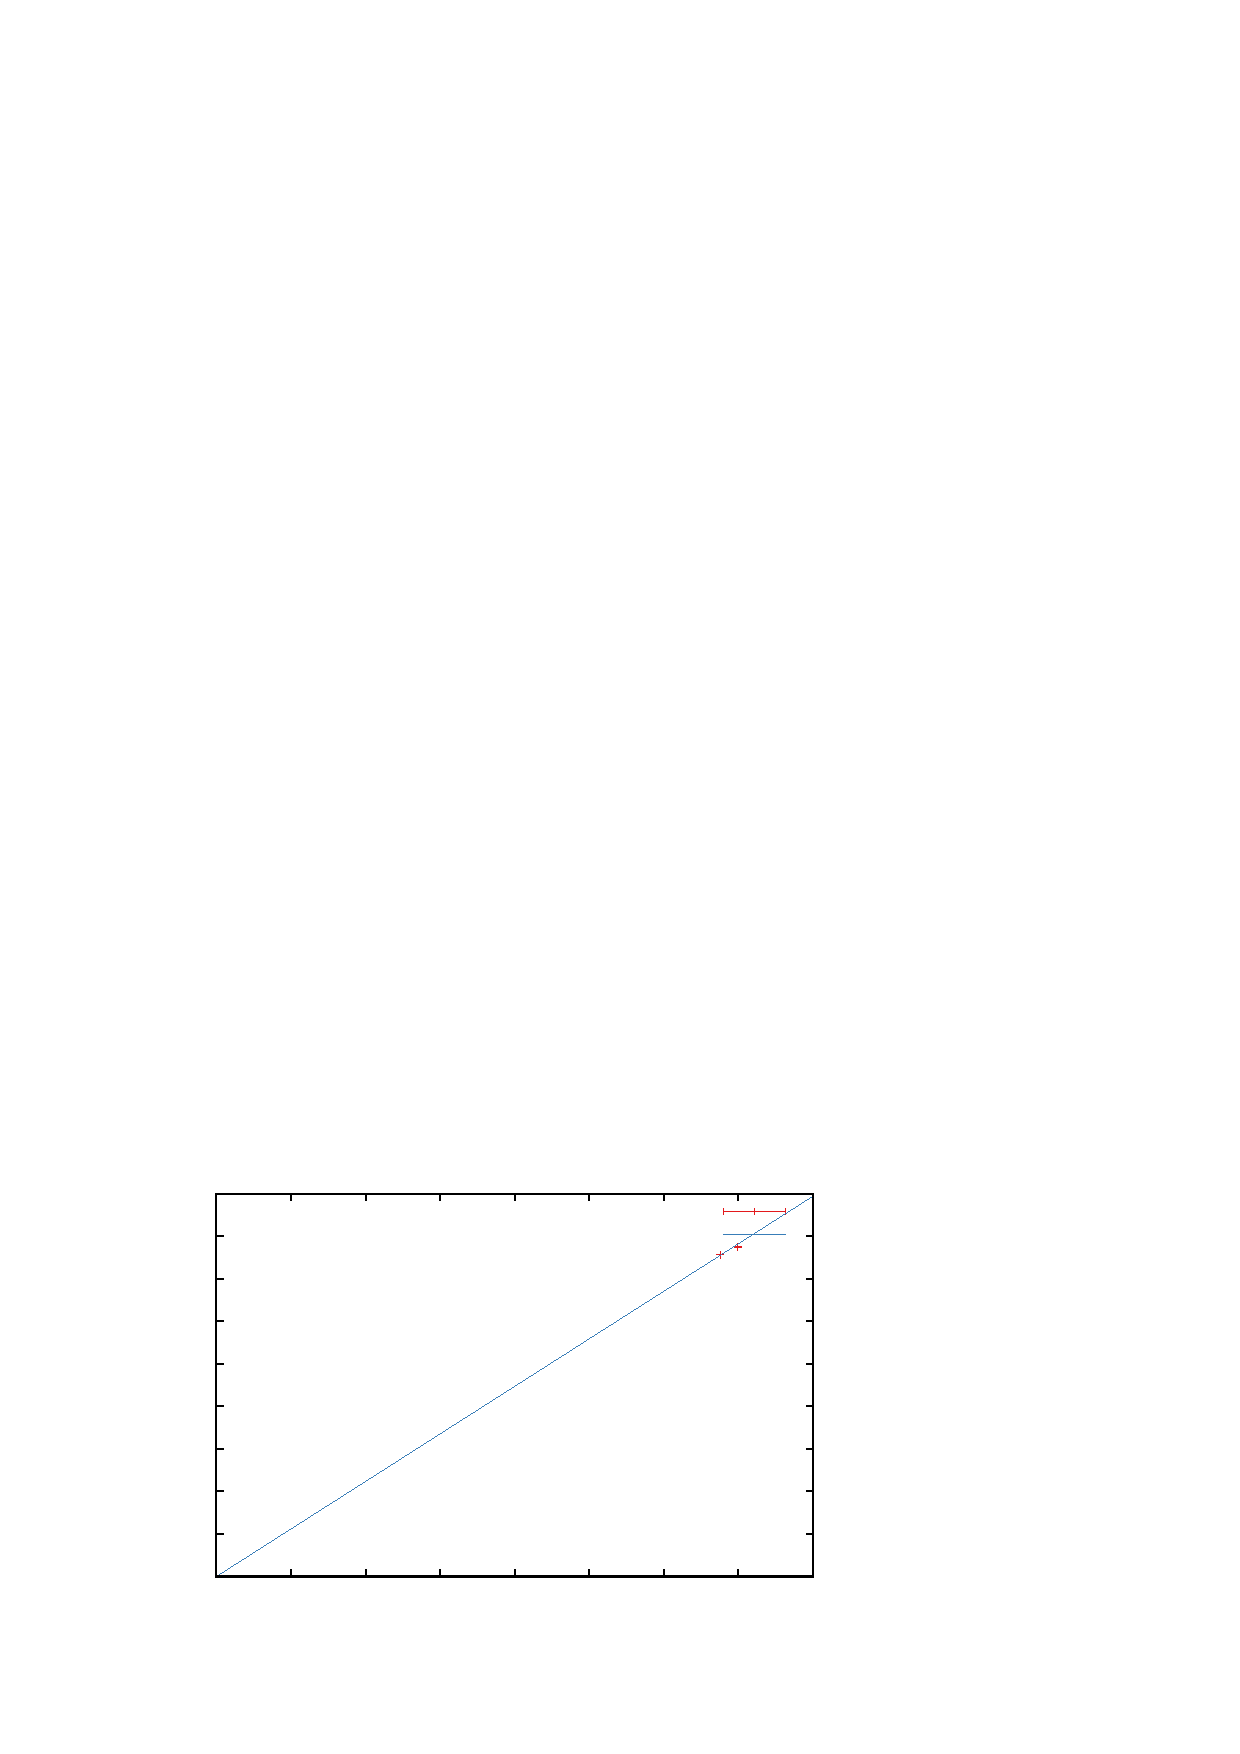
\includegraphics{./plots/kalibration}}%
    \gplfronttext
  \end{picture}%
\endgroup

	\caption{Kalibration}
	\label{fig:kalibration}
\end{figure}
\begin{align}
	\lambda \approx \SI{22.4 +- 0.1}{G.cm\per\skt}
\end{align}

\subsubsection{Feinspektrum von Barium}

\begin{table}[h]
	\centering
	\begin{tabular}{SS}
\toprule
{Messung} & {N}  \\
\midrule
1  & 6  \\
2  & 8  \\
3  & 10 \\
4  & 8  \\
5  & 5  \\
6  & 13 \\
7  & 9  \\
8  & 3  \\
9  & 9  \\
10 & 9  \\
\midrule
{$\overline{N}$} & {$\Delta N$} \\
8.0 & 2.8 \\
\bottomrule
\end{tabular}
	\caption{Untergrund \isotope[137]{Ba} bei 4}
	\label{tab:untergrund_ba4}
\end{table}
\subsection{Bestimmung der Zerfallsenergie}


\section{Fazit}

\clearpage
% BIBLIOGRAPHIE
\vspace{\fill}
% Maximale Anzahl der Einträge in Klammer
% Zitieren mit \cite{lamport94}
\begin{thebibliography}{19}
\bibitem{javan}
	A. Javan, W. R. Bennett, Jr., and D. R. Herriott,
	\emph{Population Inversion and Continuous Optical Maser Oscillation in a Gas Discharge Containing a He-Ne Mixture},
	Phys. Rev. Lett. 6, 106 – Published 1 February 1961

\bibitem{linden}
	S. Linden,
	Skript zur Vorlesung \emph{physik311: Optik und Wellenmechanik} (Stand: 31. Januar 2014),
	Physikalisches Institut, Universität Bonn

\bibitem{siegman}
	A. E. Siegman,
	\emph{Lasers},
	University Science Books 1986,
	Chapter 19: Stable Two-Mirror Resonators

\bibitem{anleitung}
	Physikalisches Praktikum V: Kern- und Teilchenphysik,
	Versuchsbeschreibung \emph{P523: $\beta$-Spektrometer} (Stand: Januar 2015),
	Universität Bonn
	
\bibitem{messschieber_katalog}
	\emph{Mitutoyo Messgeräte-Katalog},
	ABSOLUTE AOS Digimatic Messschieber,\\
	\url{http://www2.mitutoyo.de/ebooks/german/handmessgeraete/index.html} (Letzter Abruf: 22. Dezember 2014)	

\bibitem{schawlow}
	A. L. Schawlow,
	\emph{Measuring the Wavelength of Light with a Ruler},
	Am. J. Phys., Volume 33, Issue 11 (1965)

\bibitem{NISTSpectra}
	Kramida, A., Ralchenko, Yu., Reader, J., and NIST ASD Team (2014).
	\emph{NIST Atomic Spectra Database} (ver. 5.2).
	\url{http://physics.nist.gov/asd} (Letzter Abruf: 18. Dezember 2014).
	National Institute of Standards and Technology, Gaithersburg, MD.
	
\bibitem{horowitz_hill}
	Paul Horowitz, Winfred Hill,
	\emph{The Art of Electronics Second Edition},
	Cambridge University Press 1989,
	Chapter 13.12: High frequency and high-speed techniques -- Radiofrequency circuit elements

\bibitem{iupac_periodic_table}
	International Union of Pure and Applied Chemistry,
	\emph{IUPAC Periodic Table of the Elements} (Stand: 1. Mai 2013),
	\url{http://iupac.org/reports/periodic_table/}

\bibitem{meschede}
	Dieter Meschede,
	\emph{Optik, Licht und Laser} (3. Auflage),
	Vieweg Teubner 2008
	
	
 
\end{thebibliography}

\clearpage

% APPENDIX
\begin{appendix}
\section{Anhang}
\subsection{Messwerte der Photospannung hinter dem Polarisator}

\subsection{Bestimmung des Strahlprofils im Resonator}

\subsection{Bestimmung der Modenabstände mit dem optischen Spektrumanalysator}

\end{appendix}

\end{document}
